\documentclass[11pt]{article}
\usepackage[T1]{fontenc}
\usepackage[utf8]{inputenc}
\usepackage[letterpaper]{geometry}

\usepackage{graphicx}
\usepackage{mathpazo}

\usepackage{amsmath}
\usepackage{amsfonts}
\usepackage{bm}
\usepackage{siunitx}
\usepackage{cancel}
\usepackage{float}
\usepackage{empheq}
\usepackage[most]{tcolorbox}

% Sexy yellow highlighted boxed equations!
\newtcbox{\mymath}[1][]{%
	nobeforeafter, math upper, tcbox raise base,
	enhanced, colframe=black!30!black,
	colback=yellow!30, boxrule=1pt,
	#1}

% Hyperlinks with decent looking default colors.
\usepackage{hyperref}
\usepackage{xcolor}
\hypersetup{
	colorlinks,
	linkcolor={red!50!black},
	citecolor={blue!50!black},
	urlcolor={blue!80!black}
}

% For those sexy spaced low small caps from classic-thesis!
\usepackage{microtype}
\usepackage{textcase}
\DeclareRobustCommand{\spacedlowsmallcaps}[1]{%
	\textls[80]{\scshape\MakeTextLowercase{#1}}%
}

% Replaced mathpazo \sum symbol with computer modern's.
\DeclareSymbolFont{cmlargesymbols}{OMX}{cmex}{m}{n}
\let\sumop\relax
\DeclareMathSymbol{\sumop}{\mathop}{cmlargesymbols}{"50}

% Force indent command.
\newcommand{\forceindent}{\leavevmode{\parindent=1em\indent}}

% Math shortcuts.
\newcommand\p[2]{\frac{\partial #1}{\partial #2}}

% fancyhdr header and footer.
\usepackage{fancyhdr}
\pagestyle{fancy} 
\fancyhead{}
\rhead{Ali Ramadhan}
\chead{}
\lhead{12.818: Project 6}
\cfoot{}
\rfoot{\thepage}

\title{\spacedlowsmallcaps{\small 12.818: Introduction to Atmospheric Data and Large-scale Dynamics}\\ \spacedlowsmallcaps{\Large Project six: Weather fronts and the thermal wind}}
\author{\spacedlowsmallcaps{Ali Ramadhan}}
\date{}

\begin{document}
\maketitle

In this project we will investigate the structure of atmospheric fronts and the relationship between the large-scale temperature and wind fields as described by the \emph{thermal wind}. Note that the thermal wind is not actually a wind, but rather a vertically varying \emph{wind shear} that arises due to a balance between the Coriolis and pressure-gradient forces, and so it describes changes in wind with height, rather than the wind itself.

\section{Estimates of the thermal wind from instantaneous fields}

We will first look at a particularly cold weather front that passed through the Northeastern United States during mid-February 2016 when temperatures dropped to \SI{-9}{\degree F} with a record low wind chill of \SI{-36}{\degree F} in Boston, MA. Figure \ref{fig:thta_500hPa_NH} shows a contour map of the potential temperature field over the Northern Hemisphere at \SI{500}{\hecto\Pa} on February 14, 2016 (0Z) showcasing the cold frontal region and the large temperature gradient associated along the front.

\begin{figure}[h!]
	\centering
	\includegraphics[trim={0 0 3.5cm 0}, clip, width=\textwidth]{thta_500hPa_NH}
	\caption{Potential temperature field at \SI{500}{\hecto\Pa} over the Northern Hemisphere on February 14, 2016 (0Z) showcasing a particularly cold front as it is about to pass through the Northeastern United States.}
	\label{fig:thta_500hPa_NH}
\end{figure}

To investigate the cold front in more detail, we will look at cross-sectional data, and in particular data across the meridional cross-sections from the equator to the North Pole along the \SI{70}{\degree W} meridian which passes through Boston, MA at \SI{42}{\degree N} and right through the center of the cold front over Central Maine at \SI{46}{\degree N}.

Figure \ref{fig:tmpc_xsec} shows a meridional cross-section of the temperature (in \SI{}{\degreeCelsius}). As expected, the temperature decreases with height near the surface, however, with some peculiarities. In the tropics, the temperature appears to decrease roughly in accordance with the adiabatic lapse rate, and indeed the observed lapse rate is roughly constant even up to \SI{100}{\hecto\Pa}. In the high-latitudes we see a smaller lapse rate and a temperature that is nearly constant around the tropopause, dropping by only \SI{10}{\K} from \SI{325}{\hecto\Pa} to \SI{125}{\hecto\Pa}. The cold front is easily identified in the mid-latitudes by the region where several isotherms all change slope to become nearly vertical, indicating a strong temperature gradient. Interestingly, in the upper atmosphere above the cold front we see a region of nearly constant temperature, where the temperature gradient is actually much stronger in the meridional direction than the vertical.

\begin{figure}[h!]
	\centering
	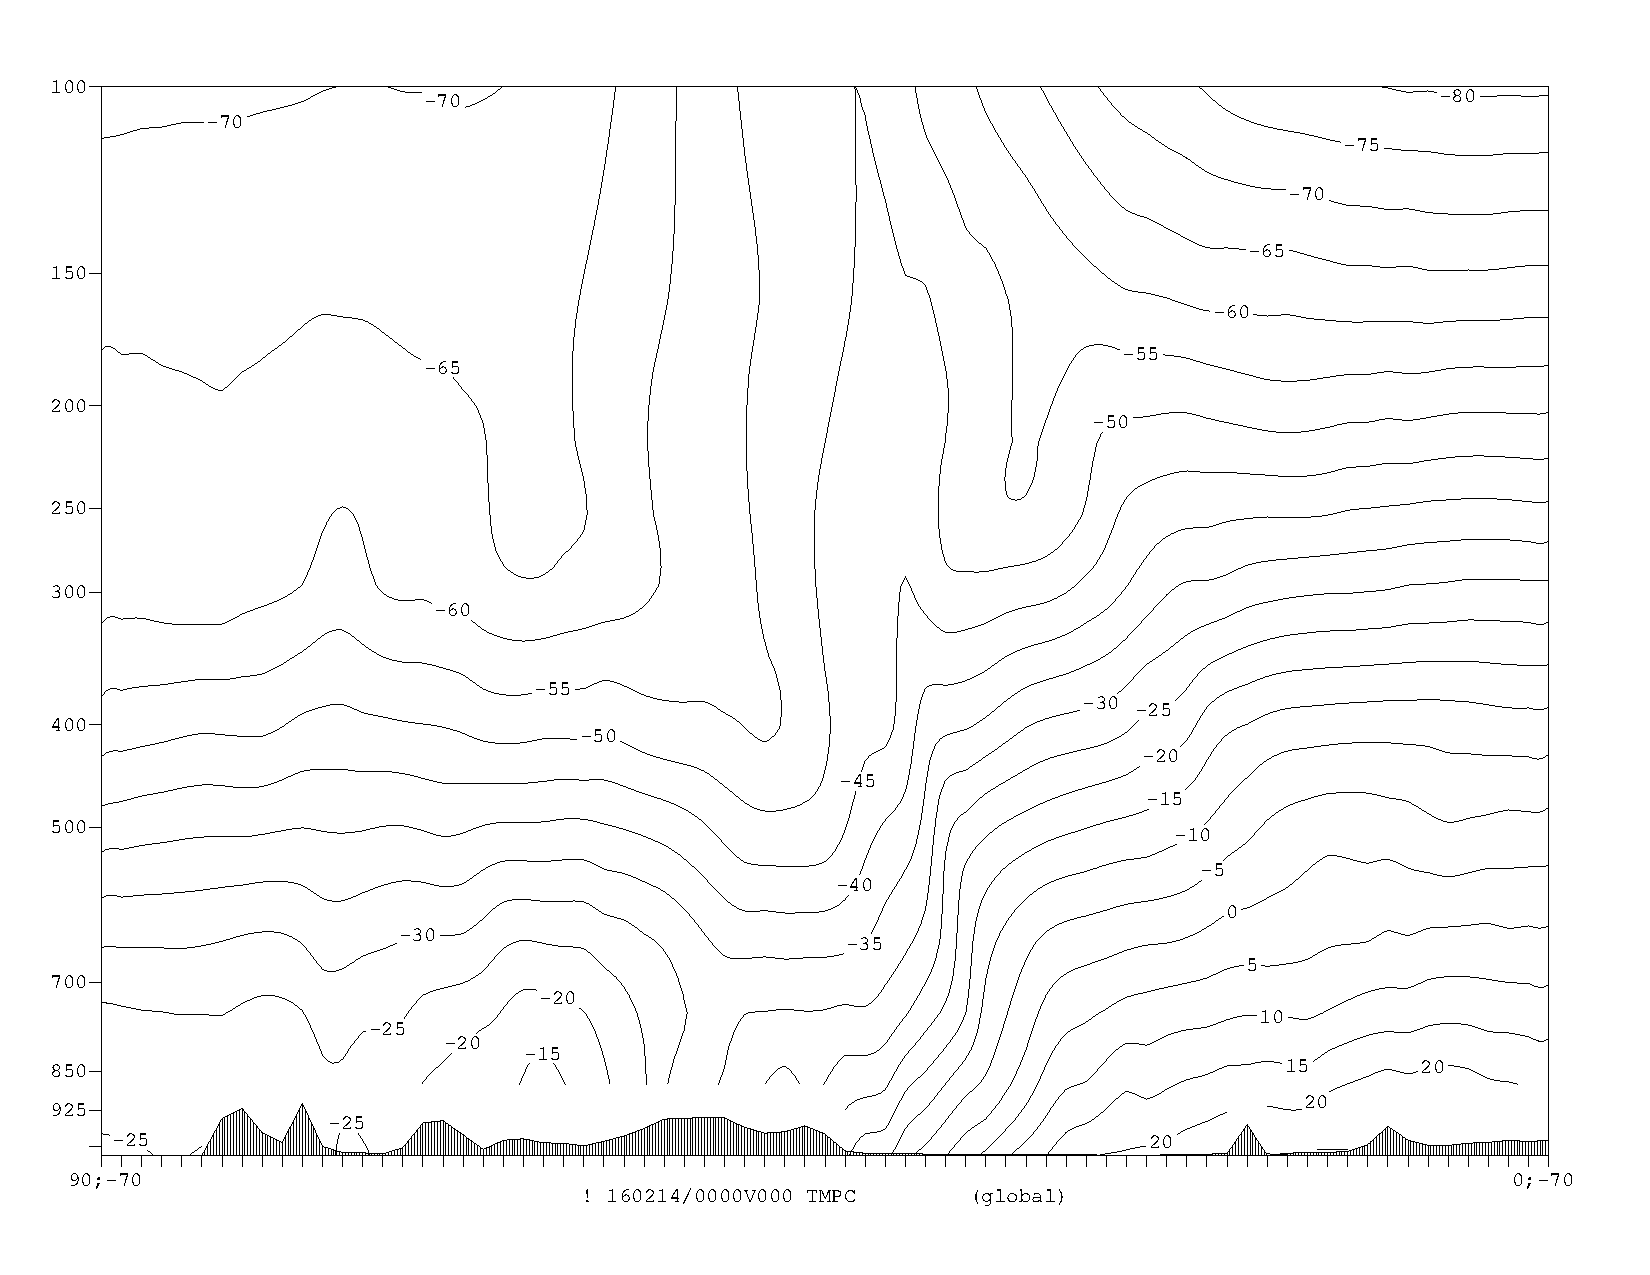
\includegraphics[width=\textwidth]{tmpc_0-90N_70W}
	\caption{Meridional cross-section of the temperature (\SI{}{\degreeCelsius}) from the equator to the North Pole along the \SI{70}{\degree W} meridian at \SI{500}{\hecto\Pa} on February 14, 2016 (0Z).}
	\label{fig:tmpc_xsec}
\end{figure}

Figure \ref{fig:thta_xsec} shows a meridional cross-section of the potential temperature $\theta$ (in \SI{}{\K}). Once again the cold front is easily identified in the mid-latitudes by the almost vertical potential temperature isotherms. We see a larger potential temperature gradient over the high-latitudes, especially in the upper atmosphere and a lower potential temperature gradient over the tropics. There is an obvious dip in potential temperature at mid-latitudes over the cold frontal region, as expected since bringing a parcel of air from the upper atmosphere down to \SI{1000}{\hecto\Pa} will bring it into the cold frontal region and the parcel's temperature will not increase as much had this been done in the tropics or at higher-latitudes.

As potential temperature is conserved in adiabatic motion, air parcels tend to flow along surfaces of constant potential temperature which can be thought of as a manifestation of the principle of minimum energy which is itself a restatement of the second law of thermodynamics. In the case of the cold front depicted in figure \ref{fig:thta_xsec}, since air parcels travel along the lines of constant potential temperature and these lines are vertical , the warm air is lifted by the cold front as it passes through and is replaced by the colder denser air making its way south from the Arctic.

\begin{figure}[h!]
	\centering
	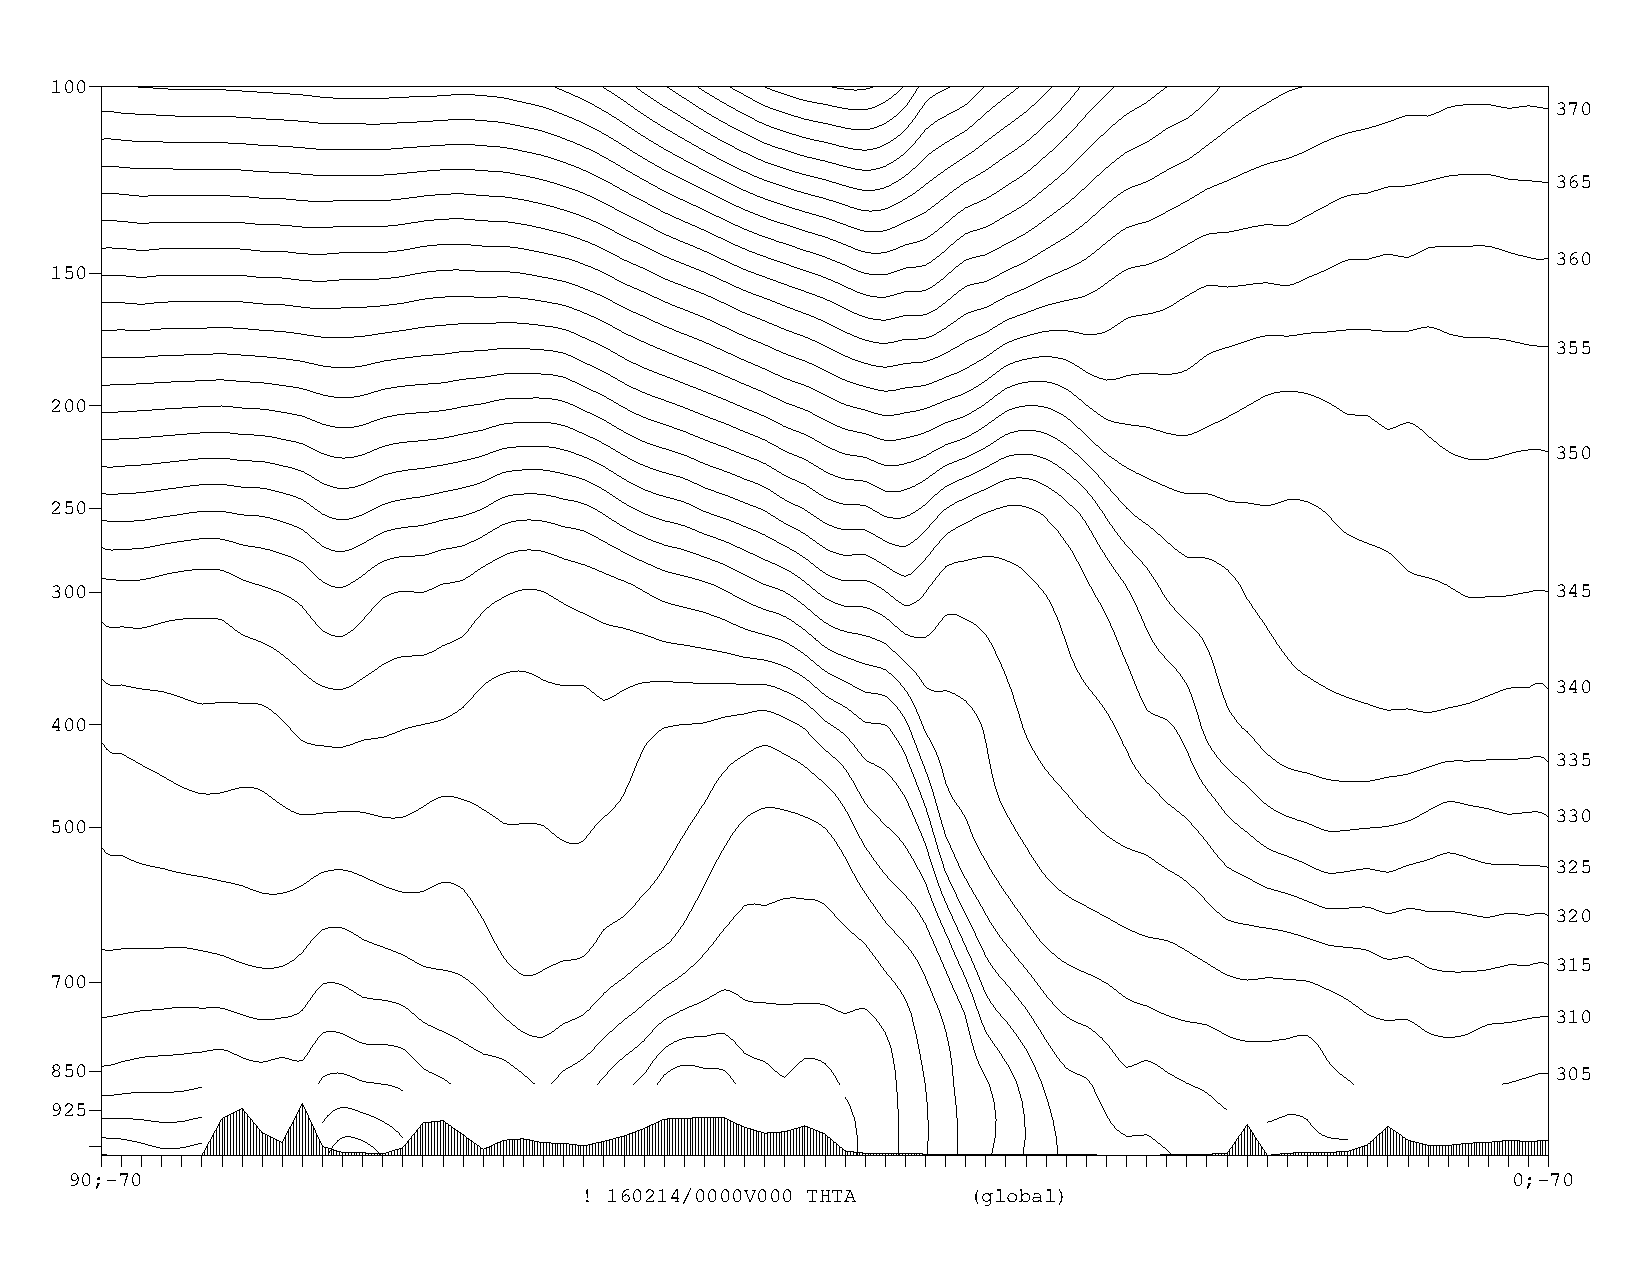
\includegraphics[width=\textwidth]{thta_0-90N_70W}
	\caption{Meridional cross-section of the potential temperature (K) from the equator to the North Pole along the \SI{70}{\degree W} meridian at \SI{500}{\hecto\Pa} on February 14, 2016 (0Z).}
	\label{fig:thta_xsec}
\end{figure}

Figure \ref{fig:thta_normwnd_xsec} now shows a meridional cross-section of the potential temperature $\theta$ (in \SI{}{\K}) along with the observed wind velocity field (normal to the cross-section) superimposed in blue. In class we saw that the thermal wind relationship can be expressed mathematically in pressure coordinates as
\begin{equation}
	\p{u}{p} = \frac{R}{fp} \left( \p{T}{y} \right)_p, \quad \p{v}{p} = -\frac{R}{fp} \left( \p{T}{x} \right)_p
\end{equation}
for a surface of constant pressure, where $\bm{u} = (u,v)$ denotes the two-dimensional wind velocity on the surface and the temperature gradients are evaluated along the surface and thus at constant pressure $p$. $R$ denotes the gas constant for a standard atmosphere and $f = 2\Omega\sin\vartheta$ is the Coriolis parameter and $\vartheta$ denotes the latitude. The $x$-coordinate represents the zonal direction while the $y$-coordinate represents the meridional. Therefore, as the thermal wind is directly proportional to the orthogonal component of the temperature gradient, we expect a strong change in the zonal wind profile meridionally along the cold front. And indeed, we do observe this. The zonal wind velocity increases from a low of around \SI{10}{\m/\s} to a peak of over \SI{50}{\m/\s} in the mid-atmosphere. The meridional temperature gradient is almost zero above the high-latitudes and thus we should expect no zonal winds there, and indeed the zonal wind profile is below \SI{10}{\m/\s} almost everywhere in the high-latitudes. The temperature profile in the tropics shows some more variability in the meridional direction and this is reflected in the zonal wind profile, which shows more variability, going up to \SI{20}{\m/\s} in some places that are still far away from the cold front. Thus it seems that the thermal wind relationship accurately predicts the vertical zonal wind profile, at least in a qualitative sense. I suppose it helps that we used a cross-sectional profile across a very prominent cold front, and the relationship may not hold as well for weaker cold fronts, or for warm fronts which tend to be weaker.

\begin{figure}[h!]
	\centering
	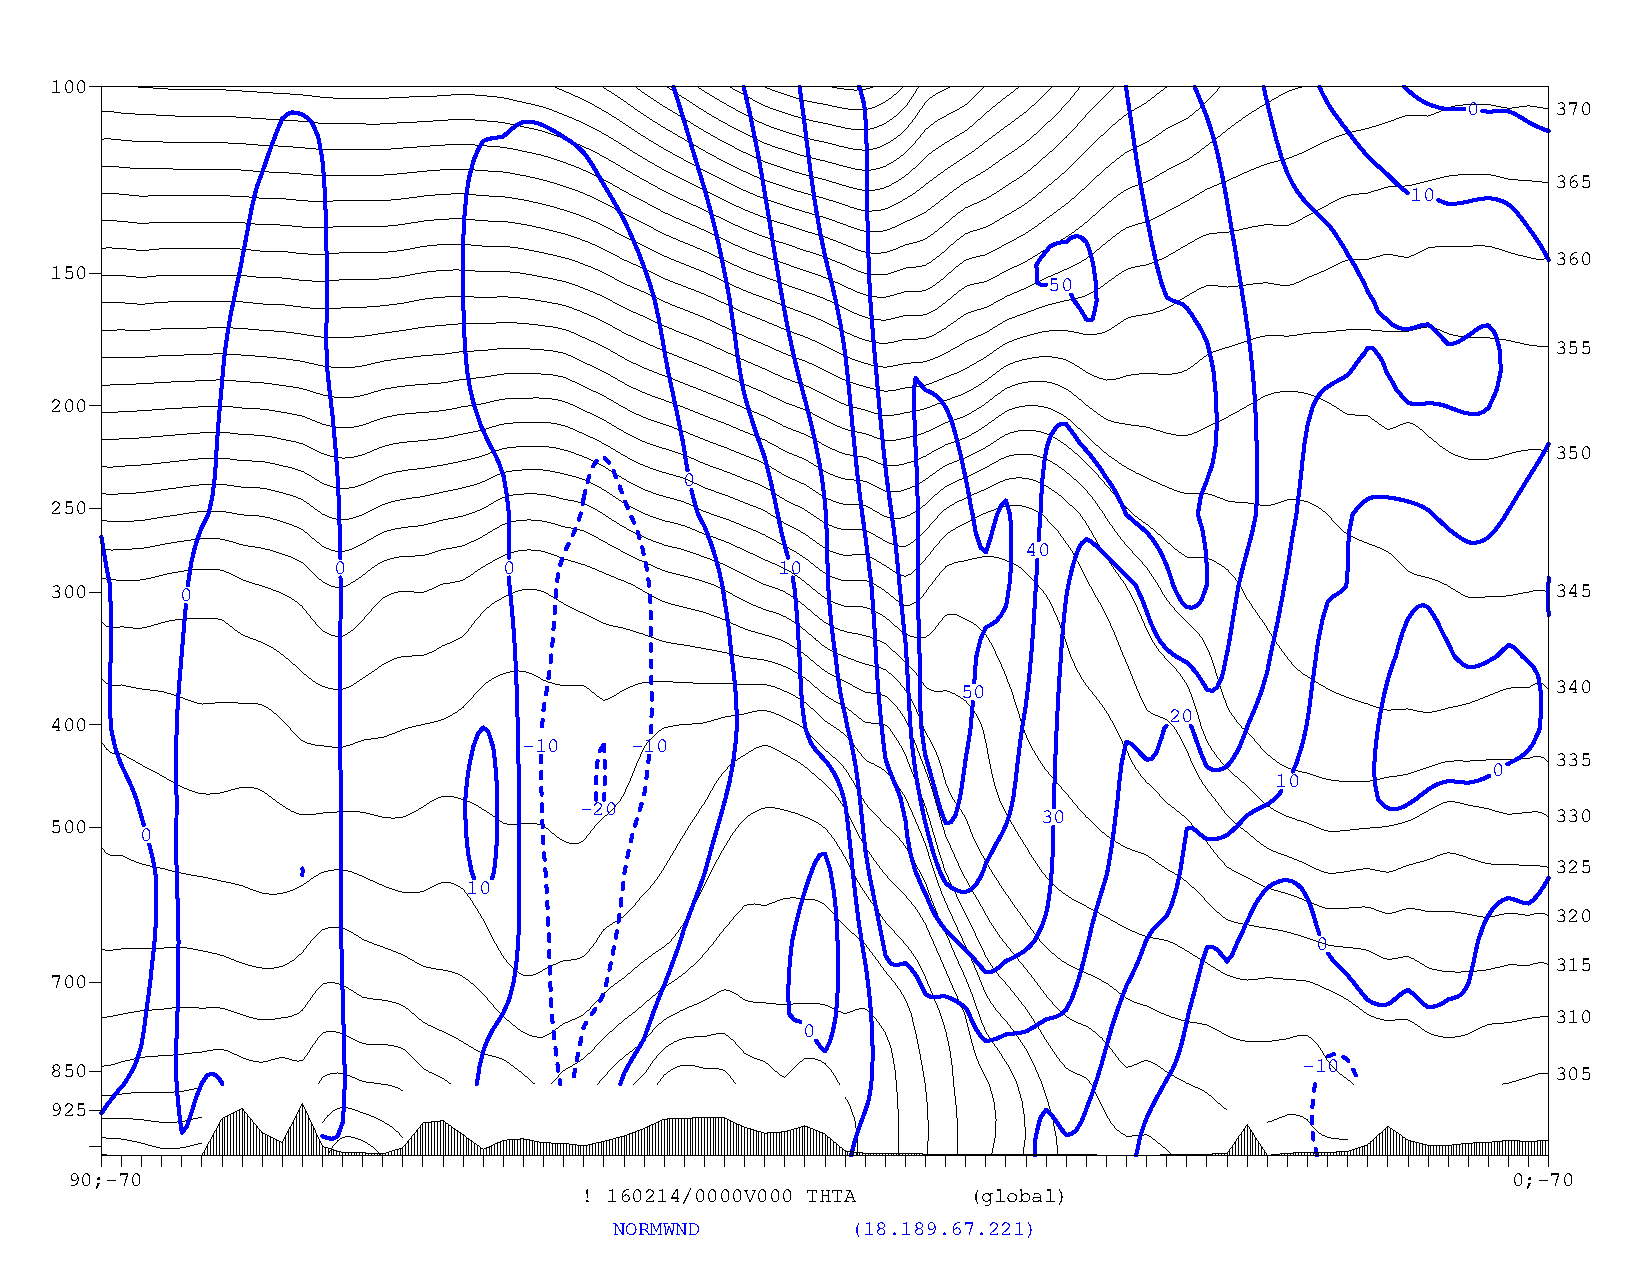
\includegraphics[width=\textwidth]{thta_normwnd_0-90N_70W}
	\caption{Meridional cross-section of the potential temperature (K) and observed wind velocity (normal to the cross-section) from the equator to the North Pole along the \SI{70}{\degree W} meridian at \SI{500}{\hecto\Pa} on February 14, 2016 (0Z).}
	\label{fig:thta_normwnd_xsec}
\end{figure}

\section{Estimates of the thermal wind from climatological fields}

Having just verified that the thermal wind relationship holds across cold weather fronts, we will attempt to verify its accuracy for the polar front using climatogical temperature and wind velocity fields for the month of July averaged over several decades. The climatological data and plots were obtained from the NCEP Reanalysis project. Figures \ref{fig:600hPa_zonal_wind_July_SH} and \ref{fig:400hPa_zonal_wind_July_SH} show contour plots of the zonal wind velocity over the Southern Hemisphere in July at \SI{600}{\hecto\Pa} and \SI{400}{\hecto\Pa}, respectively, while figure \ref{fig:500hPa_potential_temperature_July_SH} shows a contour plot of the potential temperature over the Southern Hemisphere in July at \SI{500}{\hecto\Pa} now.

\begin{figure}[h!]
	\centering
	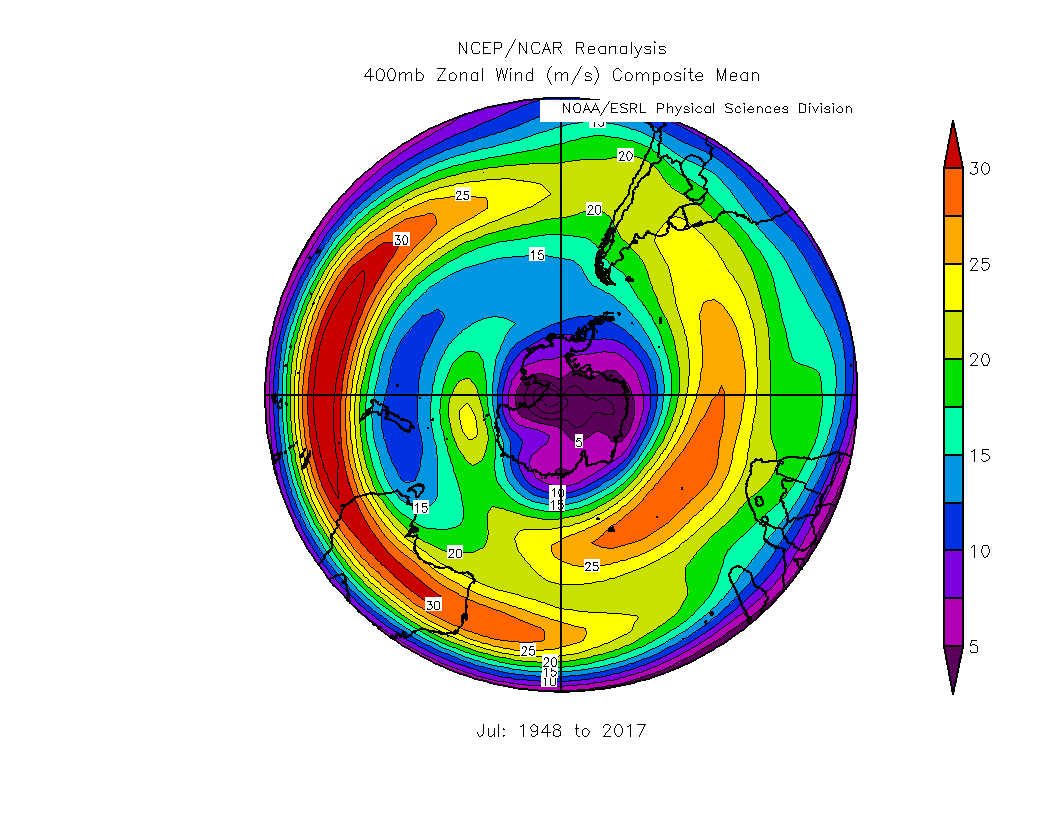
\includegraphics[width=\textwidth]{400hPa_zonal_wind_July_SH.png}
	\caption{Climatological zonal wind field at \SI{400}{\hecto\Pa} over the Southern Hemisphere during July.}
	\label{fig:400hPa_zonal_wind_July_SH}
\end{figure}

\begin{figure}[h!]
	\centering
	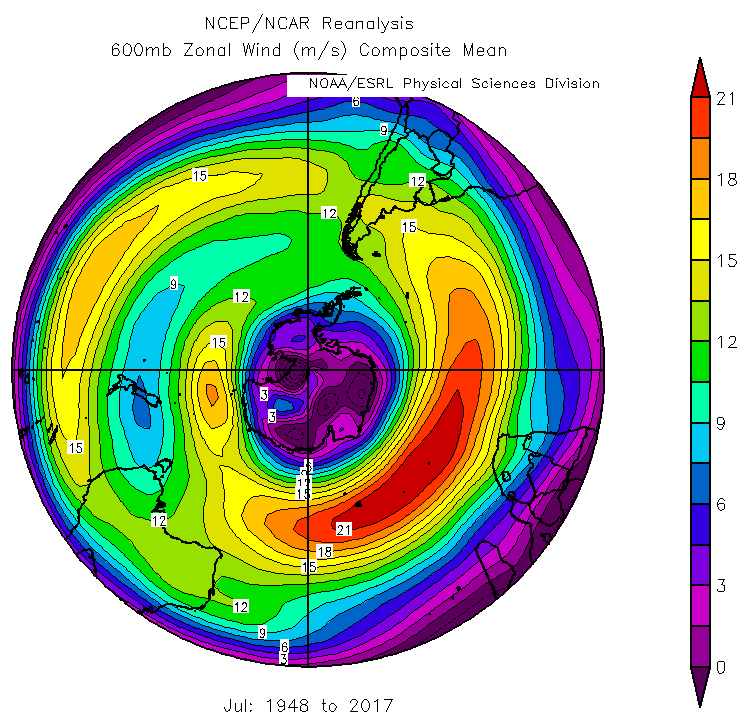
\includegraphics[width=\textwidth]{600hPa_zonal_wind_July_SH.png}
	\caption{Climatological zonal wind field at \SI{600}{\hecto\Pa} over the Southern Hemisphere during July.}
	\label{fig:600hPa_zonal_wind_July_SH}
\end{figure}

\begin{figure}[h!]
	\centering
	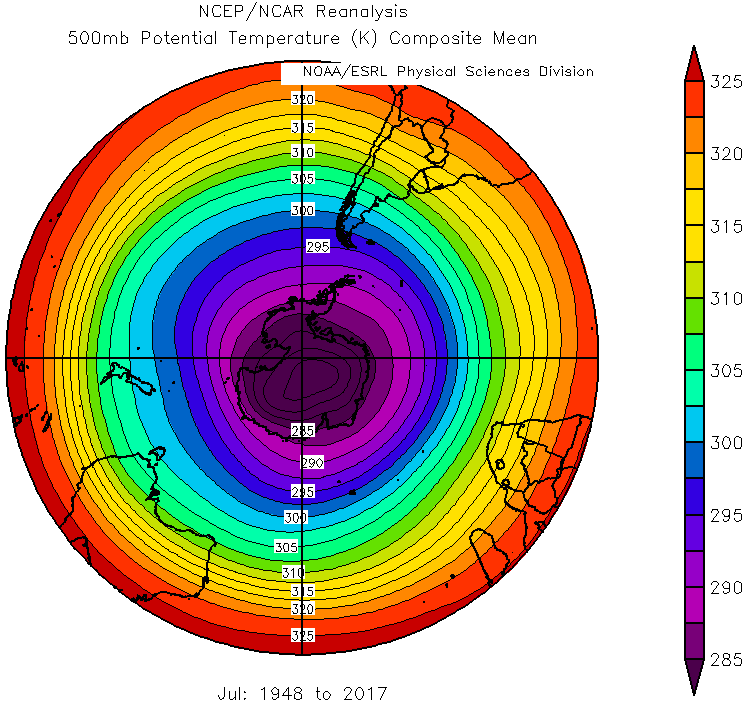
\includegraphics[width=\textwidth]{500hPa_potential_temperature_July_SH_2.png}
	\caption{Climatological potential temperature field at \SI{500}{\hecto\Pa} over the Southern Hemisphere during July.}
	\label{fig:500hPa_potential_temperature_July_SH}
\end{figure}

Using this data from the NCEP Reanalysis project, we can calculate the potential temperature gradient (figure \ref{fig:thta_gradient_climo}) along with the vertical wind shear as calculated from the thermal wind relationship along with the residual as calculated from the climatological wind velocities (figure \ref{fig:vertical_wind_shear_climo}). We will do this from the South Pole to the North Pole and average out the calculation from \SI{110}{\degree E} to \SI{150}{\degree E}.

\begin{figure}[h!]
	\centering
	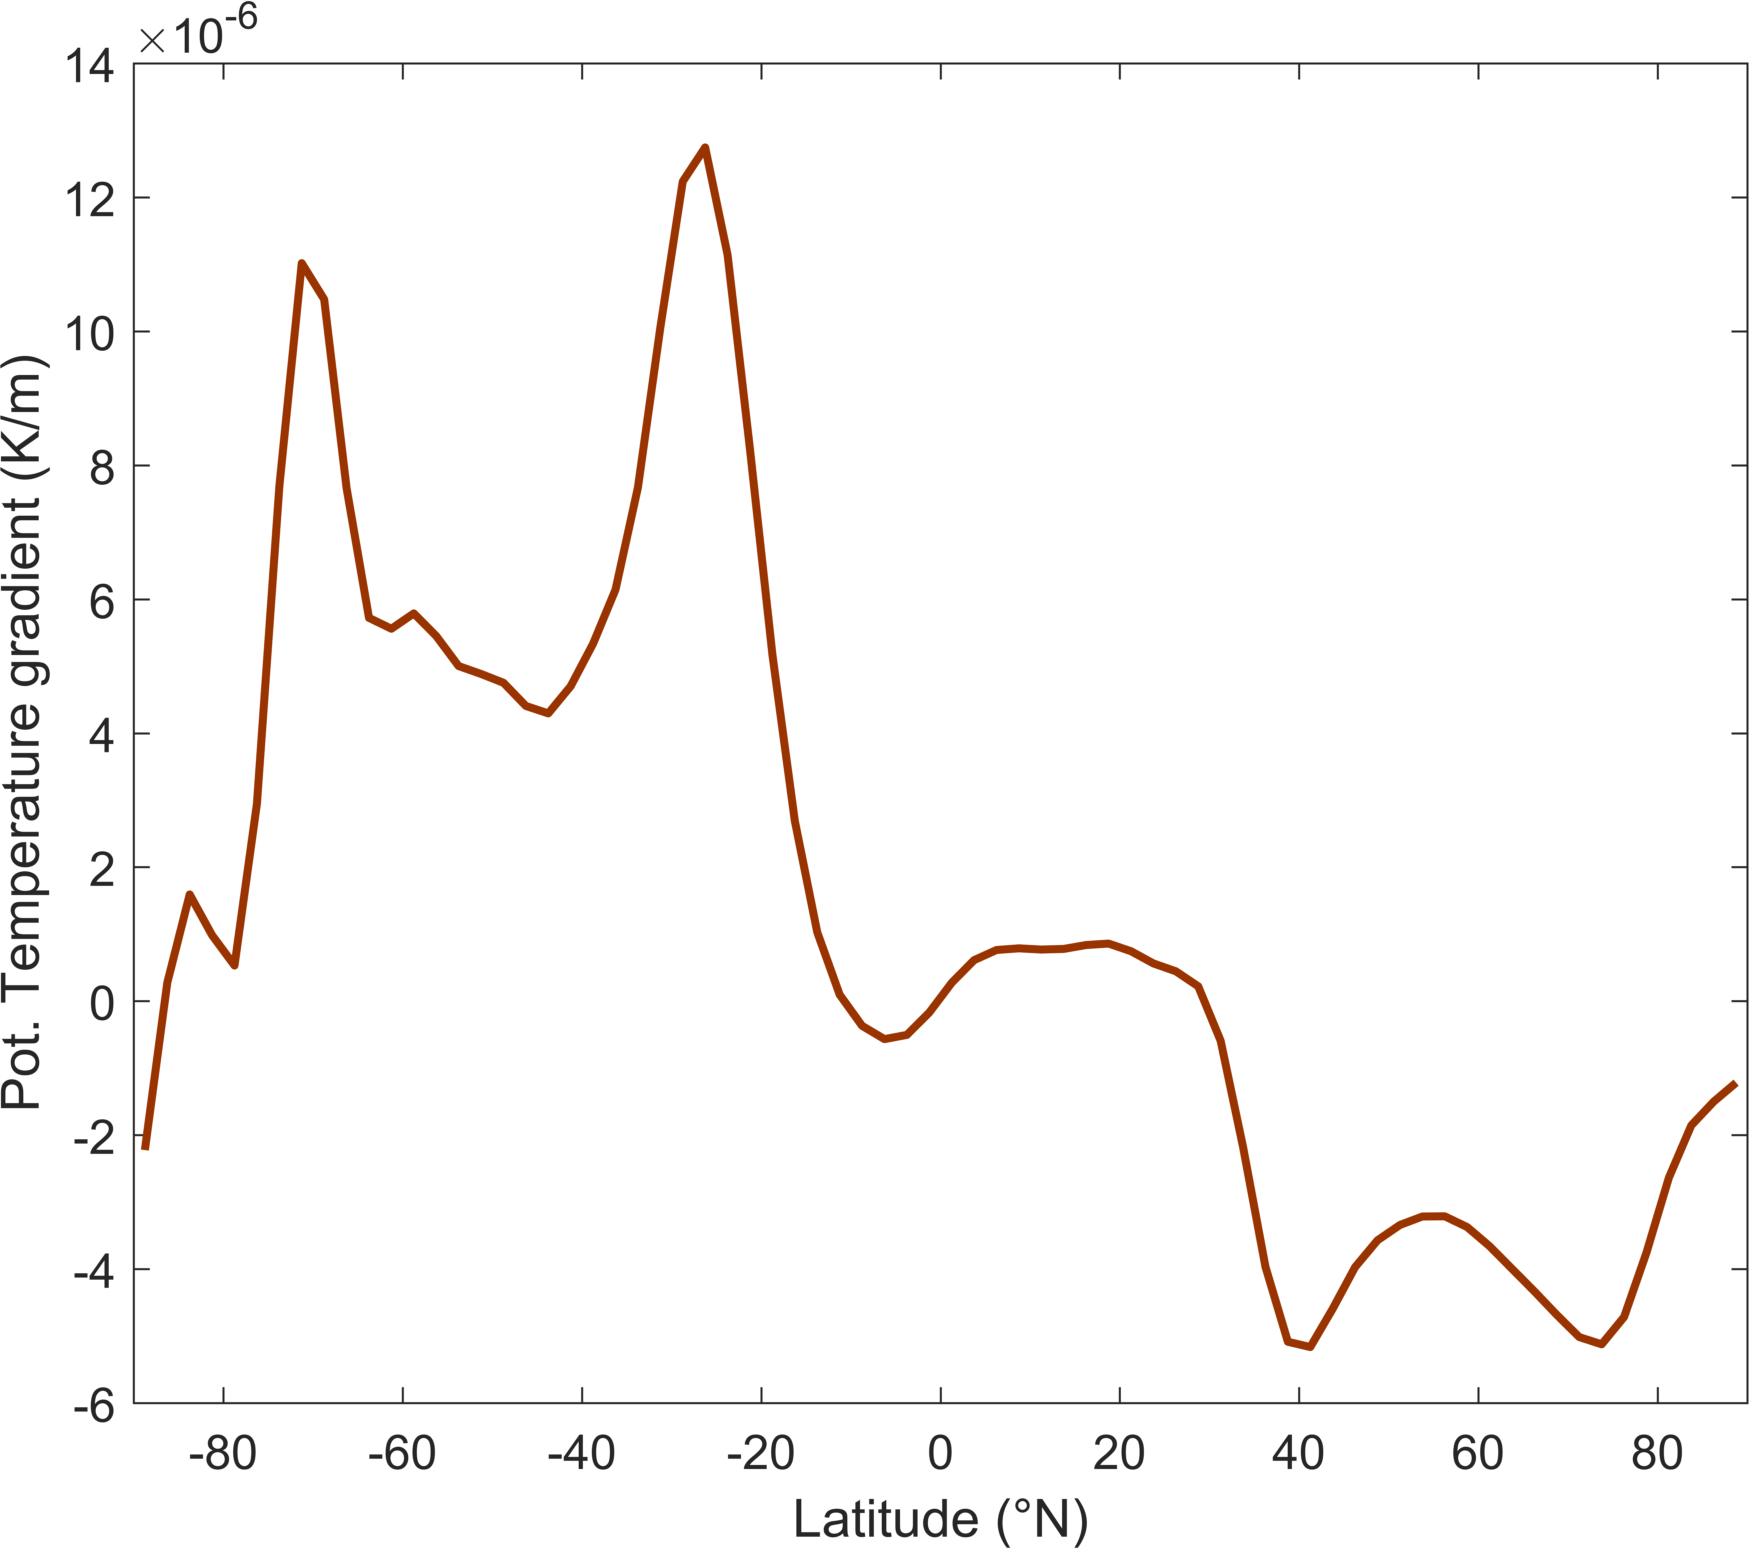
\includegraphics[width=0.7\textwidth]{thta_gradient.png}
	\caption{Potential temperature gradient (in K/m) at \SI{500}{\hecto\Pa} for the month of July from the South Pole to the North Pole, zonally averaged from \SI{110}{\degree E} to \SI{150}{\degree E}.}
	\label{fig:thta_gradient_climo}
\end{figure}

\begin{figure}[h!]
	\centering
	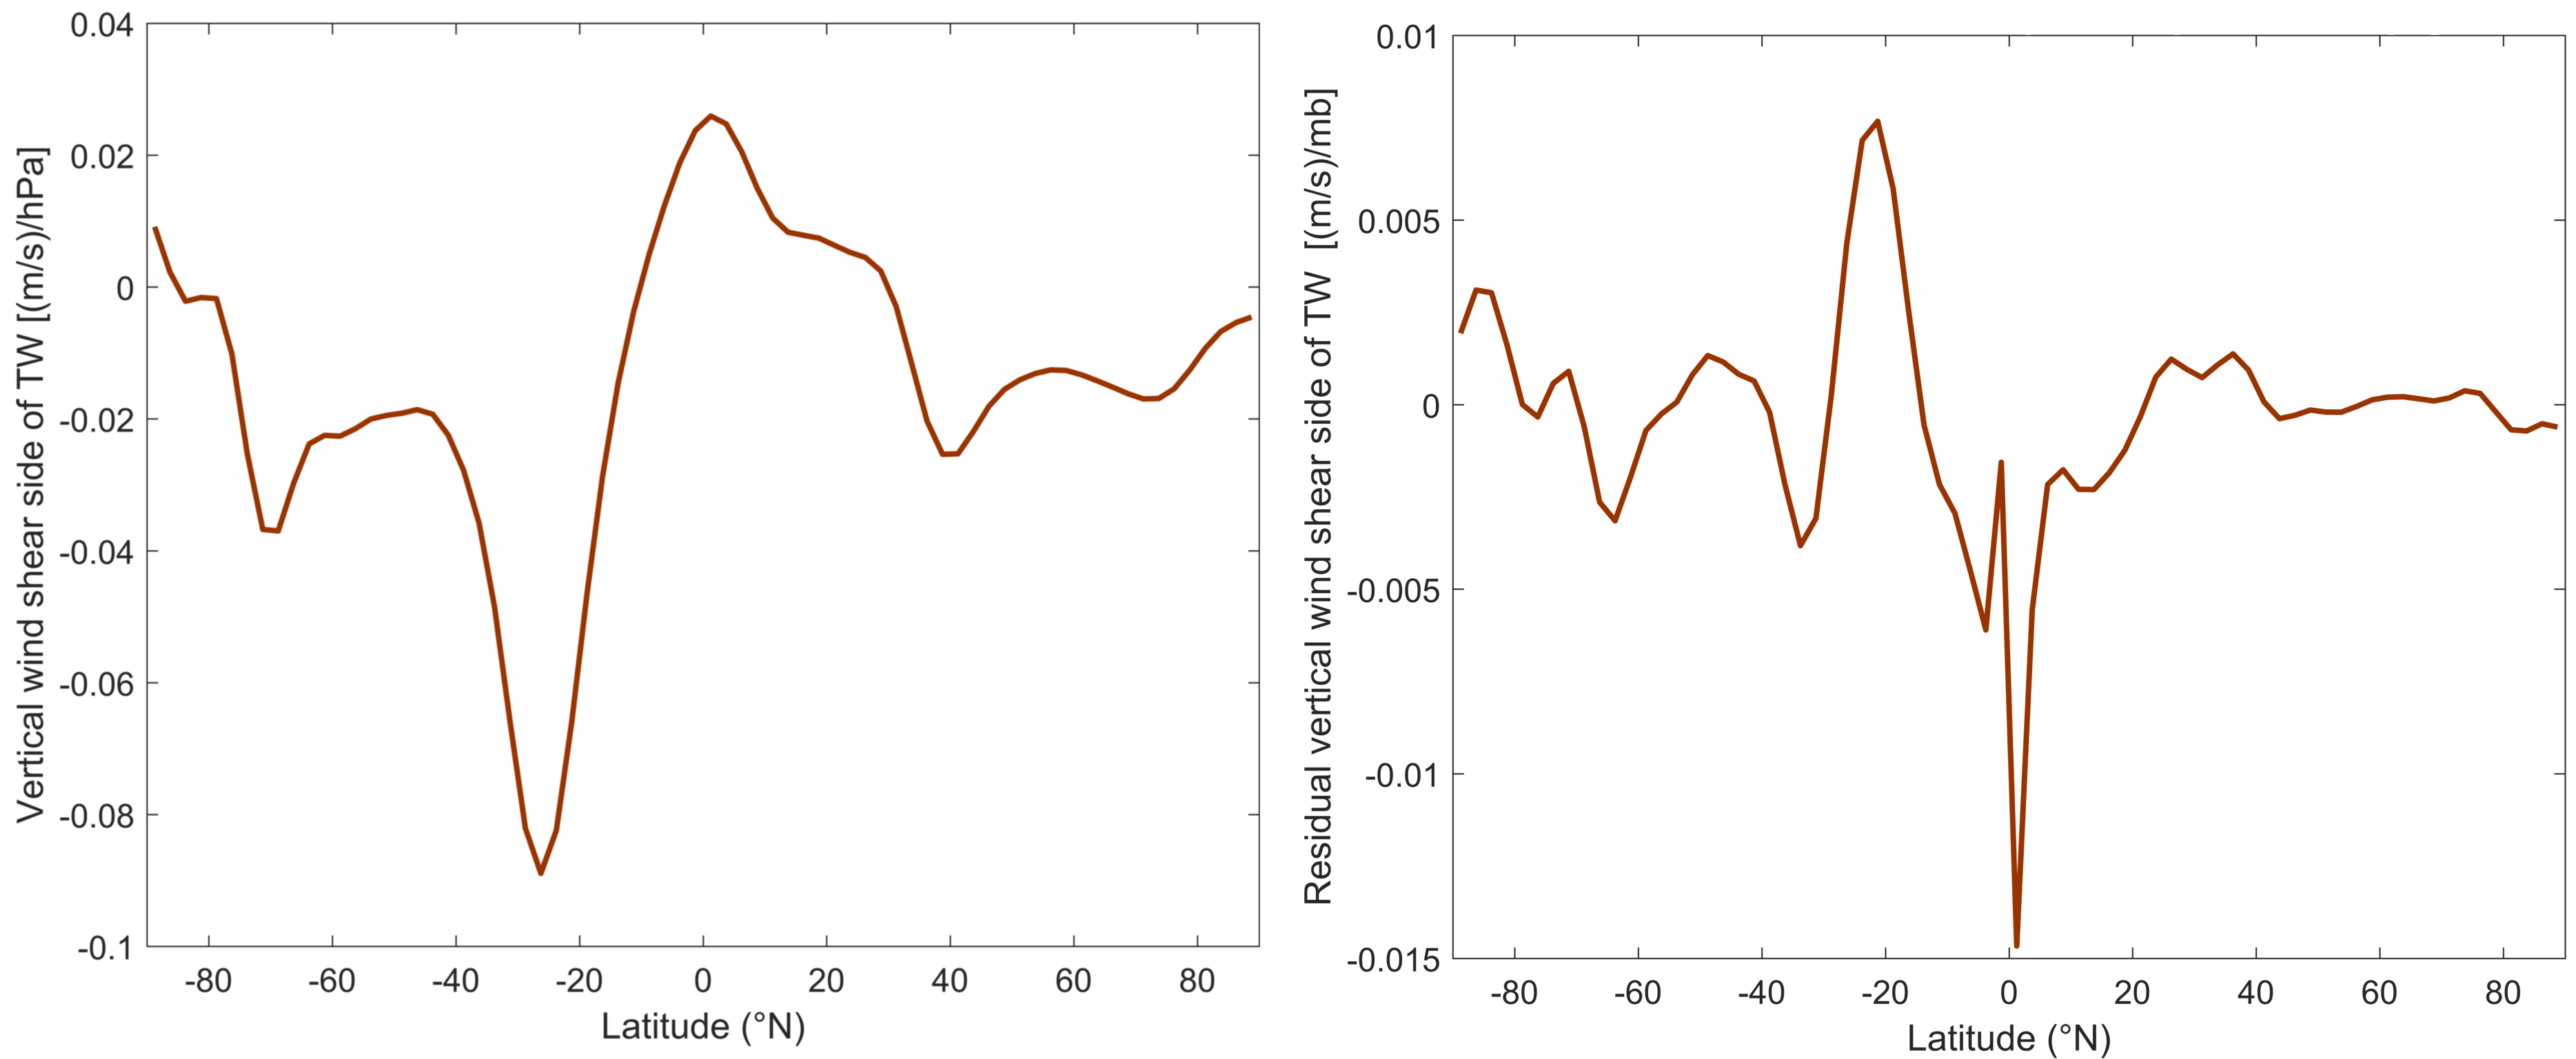
\includegraphics[width=\textwidth]{vertical_wind_shear.png}
	\caption{Climatological zonal wind field at \SI{400}{\hecto\Pa} over the Southern Hemisphere during July.}
	\label{fig:vertical_wind_shear_climo}
\end{figure}

As we saw for the cold front in the previous section, as the thermal wind balance predicts that the wind shear for the vertical zonal wind profile is proportional to the meridional temperature gradient, we should expect high zonal wind velocities in regions with high temperature gradients. Furthermore, we expect the zonal wind profile to change sign across the hemispheres. And we observe precisely that. In the Southern Hemisphere, we see two regions of high potential temperature gradient (up to \SI{12e-6}{\K/\m}) corresponding with two regions of strongly negative vertical wind shear. Interestingly, the southern polar vortex does not induce such a strong vertical wind shear as the equally strong temperature gradient near the Tropic of Capricorn around \SI{20}{\degree S}. We see weaker temperature gradients near the North Pole inducing vertical wind shears in the positive direction this time, however, the effect seems weaker than it is in the Southern Hemisphere.

It appears that thermal wind balance is indeed in effect although it does not seem to agree as strongly as it did for the case of the cold weather front from the previous section, however we did no quantitative analysis in the previous section. The residual vertical wind shear suggests that thermal wind balance accounts for the majority of the observed vertical wind shear, especially near the poles. The largest residuals appear at the equator with roughly the same order as the vertical wind shear itself. Perhaps thermal wind balance is a better approximation near the poles where temperature gradients are much higher than at the equator where the temperature gradients are lower, thus leading to the slight breakdown of thermal wind balance.

\end{document}